\pagebreak
\section{Serveur}
\label{chapter:api}

% TODO Qoi parler ?
% PARTIE API
% 1. Architecture
% 2. Points clés de l'implémentation
% 2.1 OAS : Pourquoi / utilité / example (documentation)
% 2.2 ORM : scopes query - retrieve ?
% 2.3 Sécurité : middelware
% 2.4 Configuration variable environnement

Cette section est entièrement dédiée à la conception du \gls{backend} de \texttt{SourceCode}.
Puisque cette partie est l'extrême opposée de la précédente (cf section \ref{chapter:client}), nous l'aborderons par sa réalisation technique.
Étant donné qu'une présentation exhaustive serait une tâche chronophage, nous nous concentrerons sur l'essentiel.

\subsection{Structure du projet}

Pour répondre aux besoins exprimés en chapitre \ref{chapter:analyseDesBesoins} et sur base de nos choix (cf section \ref{section:choixTechnologiques}), nous avons élaboré la présente structure :

% Généré avec tree sur Windows et https://carbon.now.sh/
\begin{figure}[H]
    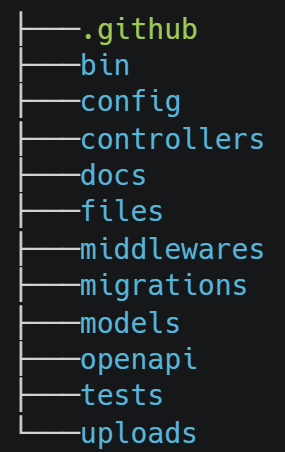
\includegraphics[width=\textwidth,height=0.25\textheight,keepaspectratio]{images/serveur/tree_folders.png}
    \centering
    \caption[SourceCode : Arborescence de l\'API]{Arborescence de \Gls{api}}
    \label{fig:arborenceAPI}
\end{figure}

Cette structure ne vous est peut-être pas inconnue, car il s'agit de la structure officielle de Sequelize\footnote{
    \url{https://github.com/sequelize/cli} - command "sequelize init"
}, sur laquelle nous avons ajouté quelques dossiers :

% A voir s'il faut minimiser l'itemize
% nosep,noitemsep,topsep=0pt,partopsep=0pt,after=\vspace*{2pt}
\begin{itemize}
    \item openapi : nos fichiers \Gls{oas}, utilisés par openapi-enforcer (cf figure \ref{fig:OASEnforcer})
    \item controllers : nos fichiers chargés de répondre aux requêtes \textbf{HTTP}, utilisés par openapi-enforcer (cf figure \ref{fig:OASEnforcer})
    \item tests : nos tests pour valider l'implémentation (cf chap TODO)
    \item upload / files : resp. lieu de stockage des fichiers importés / stockés 
    \item .github : nos scripts d'automatisation (cf section TODO) 
    \item bin : du code n'entrant dans aucun autre dossier
\end{itemize}


\subsection{Points clés de l'implémention}

\subsubsection{Paramétrisation de \Gls{api}}
\subsubsection{\Gls{oas}}
\subsubsection{\Gls{middleware}}
\subsubsection{Recherche par \glspl{tag}}

\ref{code:searchTags}

% DIVERS
% - Docker (en annexe, les deux docker-compose)
% - CLI : max une page ou deux (expliquer ce qu'il y a dedans, en ref l'annexe A)
\section{Divers}
\label{chapter:solutionDivers}

\subsection{\texorpdfstring{\Gls{cli}}{CLI}}
\subsection{Docker}
\subsection{}


% Pas besoin d'expliquer tout , seulement l'essentiel : 
% - OpenAPI (introduit dans les choix) mais montrer la validation/doc/etc
% - Les middelwares ( securité, validation, etc... )
% - ORM 